%%%%%%%%%%%%%%%%%%%%%%%%%%%%%%%%%%%%%%%%%
% Tufte Essay
% LaTeX Template
% Version 2.0 (19/1/19)
%
% This template originates from:
% http://www.LaTeXTemplates.com
%
% Authors:
% The Tufte-LaTeX Developers (https://www.ctan.org/pkg/tufte-latex)
% Vel (vel@LaTeXTemplates.com)
%
% License:
% Apache License, version 2.0
%
%%%%%%%%%%%%%%%%%%%%%%%%%%%%%%%%%%%%%%%%%

%----------------------------------------------------------------------------------------
%	PACKAGES AND OTHER DOCUMENT CONFIGURATIONS
%----------------------------------------------------------------------------------------

\documentclass[a4paper]{tufte-handout} % Use A4 paper by default, remove 'a4paper' for US letter

\usepackage{graphicx} % Required for including images
\setkeys{Gin}{width=\linewidth, totalheight=\textheight, keepaspectratio} % Default images settings
\graphicspath{{Figures/}{./}} % Specifies where to look for included images (trailing slash required)

\usepackage{amsmath, amsfonts, amssymb, amsthm} % For math equations, theorems, symbols, etc
\usepackage{units} % Non-stacked fractions and better unit spacing

\usepackage{booktabs} % Required for better horizontal rules in tables

%----------------------------------------------------------------------------------------
%	TITLE SECTION
%----------------------------------------------------------------------------------------

\title{An Essay Worthy of a Title}

\author{Doug Rattmann}

\date{\today} % Date, use \date{} for no date

%----------------------------------------------------------------------------------------
\pagecolor{black}
\color{white}
\begin{document}

\maketitle % Print the title section

%----------------------------------------------------------------------------------------
%	ABSTRACT/SUMMARY
%----------------------------------------------------------------------------------------

\begin{abstract}
	\textbf{Summary}
	Morbi tempor congue porta. Proin semper, leo vitae faucibus dictum, metus mauris lacinia lorem, ac congue leo felis eu turpis. Sed nec nunc pellentesque, gravida eros at, porttitor ipsum. Praesent consequat urna a lacus lobortis ultrices eget ac metus. In tempus hendrerit rhoncus.
\end{abstract}

%----------------------------------------------------------------------------------------
%	ESSAY BODY
%----------------------------------------------------------------------------------------

\section{Paragraphs \& Notes}\label{sec:notes}

Lorem ipsum dolor sit amet, consectetur adipiscing elit. Praesent porttitor arcu luctus, imperdiet urna iaculis, mattis eros\footnote{One of the most prominent and distinctive features of this style is the extensive use of side notes. There is a wide margin to provide ample room for side notes and small figures. Side notes can be created using the standard \texttt{\textbackslash footnote} command or using the custom \texttt{\textbackslash sidenote} command and are automatically numbered.}. Pellentesque iaculis odio vel nisl ullamcorper, nec faucibus ipsum molestie. Sed dictum nisl non aliquet porttitor. Etiam vulputate arcu dignissim, finibus sem et, viverra nisl. Aenean luctus congue massa, ut laoreet metus ornare in. Nunc fermentum nisi imperdiet lectus tincidunt vestibulum at ac elit. Nulla mattis nisl eu malesuada suscipit.

Aliquam arcu turpis, ultrices sed luctus ac, vehicula id metus. Morbi eu feugiat velit, et tempus augue. Proin ac mattis tortor. Donec tincidunt, ante rhoncus luctus semper, arcu lorem lobortis justo, nec convallis ante quam quis lectus.\marginnote{Ancillary information can be placed in the margin using the \texttt{\textbackslash marginnote} command. Margin notes are unnumbered in the text where they are added and in the margin.} Aenean tincidunt sodales massa, et hendrerit tellus mattis ac. Sed non pretium nibh. Donec cursus maximus luctus. Vivamus lobortis eros et massa porta porttitor.

\begin{quote}
	``Some trees flourish, others die. Some cattle grow strong, others are taken by wolves. Some men are born rich enough and dumb enough to enjoy their lives. Ain't nothing fair.'' --- John Marston, 1911
\end{quote}

Fusce varius orci ac magna dapibus porttitor. In tempor leo a neque bibendum sollicitudin\sidenote{The \texttt{\textbackslash sidenote} command can take two optional arguments as follows: \texttt{\textbackslash sidenote[<number>][<offset>]\{<text>\}}}. Nulla pretium fermentum nisi, eget sodales magna facilisis eu. Praesent aliquet nulla ut bibendum lacinia. Donec vel mauris vulputate, commodo ligula ut, egestas orci. Suspendisse commodo odio sed hendrerit lobortis. Donec finibus eros erat, vel ornare enim mattis et. Donec finibus dolor quis dolor tempus consequat\sidenote[39]{This side note has a custom number using the \texttt{<number>} parameter.}.

In hac habitasse platea dictumst. Curabitur mattis elit sit amet justo luctus vestibulum. In hac habitasse platea dictumst. Pellentesque lobortis justo enim, a condimentum massa tempor eu. Ut quis nulla a quam pretium eleifend nec eu nisl. Nam cursus porttitor eros, sed luctus ligula convallis quis. Nam convallis, ligula in auctor euismod, ligula mauris fringilla tellus, et egestas mauris odio eget diam. Praesent sodales in ipsum eu dictum\sidenote[][-24pt]{This side note has been moved up using the \texttt{<offset>} argument. Positive offsets move down, negative move up. This is useful if notes clash with other margin content.}.

Maecenas consectetur metus at tellus finibus condimentum. Proin arcu lectus, ultrices non tincidunt et, tincidunt ut quam. Integer luctus posuere est, non maximus ante dignissim quis. Nunc a cursus erat. Curabitur suscipit nibh in tincidunt sagittis. Nam malesuada vestibulum quam id gravida. Proin ut dapibus velit. Vestibulum eget quam quis ipsum semper convallis. Duis consectetur nibh ac diam dignissim, id condimentum enim dictum. Nam aliquet ligula eu magna pellentesque, nec sagittis leo lobortis. Aenean tincidunt dignissim egestas. Morbi efficitur risus ante, id tincidunt odio pulvinar vitae.\marginnote[-2cm]{Margin notes can also take an \texttt{<offset>} argument to move them up or down. This margin note has been moved up to avoid clashing with the text below.}

%------------------------------------------------

\section{Full-width Text Blocks}\label{sec:fullwidthtextblocks}

\begin{fullwidth}
	\small\itshape Lorem ipsum dolor sit amet, consectetur adipiscing elit. Praesent porttitor arcu luctus, imperdiet urna iaculis, mattis eros. Pellentesque iaculis odio vel nisl ullamcorper, nec faucibus ipsum molestie. Sed dictum nisl non aliquet porttitor. Etiam vulputate arcu dignissim, finibus sem et, viverra nisl. Aenean luctus congue massa, ut laoreet metus ornare in. Nunc fermentum nisi imperdiet lectus tincidunt vestibulum at ac elit. Nulla mattis nisl eu malesuada suscipit. Aliquam arcu turpis, ultrices sed luctus ac, vehicula id metus. Morbi eu feugiat velit, et tempus augue. Proin ac mattis tortor. Donec tincidunt, ante rhoncus luctus semper, arcu lorem lobortis justo, nec convallis ante quam quis lectus. Aenean tincidunt sodales massa, et hendrerit tellus mattis ac. Sed non pretium nibh. Donec cursus maximus luctus. Vivamus lobortis eros et massa porta porttitor.
\end{fullwidth}

%------------------------------------------------

\section{Section Types}\label{sec:sectiontypes}

This style provides \textsc{a}- and \textsc{b}-heads (that is, \texttt{\textbackslash section} and \texttt{\textbackslash subsection}) only. The Tufte-\LaTeX\ classes will emit an error if you try to use \texttt{\textbackslash subsubsection} and smaller headings.

%------------------------------------------------

\section{Referencing}\label{sec:referencing}

\subsection{Referencing Sections}

Sections can be referenced by name using the \texttt{\textbackslash nameref} command, provided they have been given a label with \texttt{\textbackslash label}. For example, we can output the name of the first section in this document\sidenote{Section names output in this way are clickable links that take the reader to the section.} using its label\sidenote{\texttt{\textbackslash label\{sec:notes\}}} like this: \nameref{sec:notes}.

\subsection{Referencing Citations}

References are placed alongside their citations as side notes\cite{Tufte1997}. This is accomplished using the normal \texttt{\textbackslash cite} command. The complete list of references (i.e. bibliography) may be printed automatically using the \texttt{\textbackslash bibliography} command.

To enter multiple citations at one location\cite{Tufte2006,Tufte1990}, you can provide a list of keys separated by commas: \texttt{\textbackslash cite\{Tufte2006,Tufte1990\}}. You can also use the same optional vertical \texttt{<offset>} argument to move them up or down: \texttt{\textbackslash cite[<offset>]\{<bibkey1,bibkey2,\ldots>\}}.

%------------------------------------------------

\section{Figures \& Tables}\label{sec:figuresandtables}

The standard \texttt{figure} and \texttt{tabular} environments are available to place your figure or table within the text body with the caption appearing in the margin. Full-width figures and tables may be placed in \textsf{figure*} or \textsf{table*} environments with captions again appearing in the margin. Figure~\ref{fig:fullfig} is an example of the \texttt{figure*} environment and Figure~\ref{fig:textfig} is an example of the normal \texttt{figure} environment.

\begin{figure*}[h]
	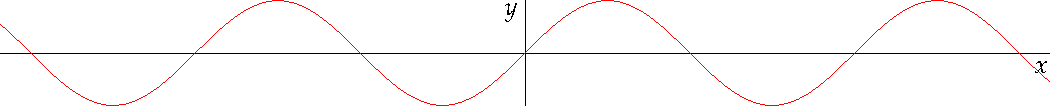
\includegraphics[width=\linewidth]{sine.pdf}%
	\caption{This graph shows $y = \sin x$ from about $x = [-10, 10]$.
	\emph{Notice that this figure takes up the full page width.}}%
	\label{fig:fullfig}%
\end{figure*}

\begin{figure}[h]
	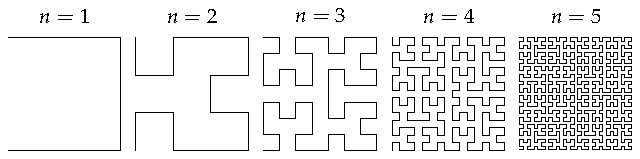
\includegraphics{hilbertcurves.pdf}
	\caption{Hilbert curves of various degrees $n$.
	\emph{Notice that this figure only takes up the main textblock width.}}
	\label{fig:textfig}
	\setfloatalignment{a} % Position the figure caption in the middle of the figure
\end{figure}

The style contains two new environments called \textsf{marginfigure} and \textsf{margintable} which allow you to place a figure or table entirely in the margin. Like side and margin notes, the \textsf{marginfigure} and \textsf{margintable} environments accept an optional \texttt{<offset>} argument that adjusts the vertical position of the figure or table. Figure~\ref{fig:marginfig} is an example of a margin figure that has been moved up due to a clash with Figure~\ref{fig:textfig} above it.

\begin{marginfigure}[-0.75cm]
	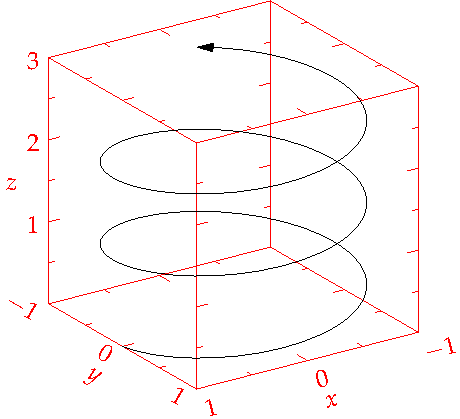
\includegraphics[width=\linewidth]{helix.pdf}
	\caption{This is a margin figure. The helix is defined by $x = \cos(2\pi z)$, $y = \sin(2\pi z)$, and $z = [0, 2.7]$. The figure was drawn using Asymptote (\url{http://asymptote.sf.net/}).}
	\label{fig:marginfig}
\end{marginfigure}

Table~\ref{tab:normaltab} shows a table created with the \texttt{booktabs} package. Notice the lack of vertical rules---they serve only to clutter the table's data.

\begin{table}[ht]
	\centering
	\fontfamily{ppl}\selectfont
	\begin{tabular}{l l}
		\toprule
		Margin & Length \\
		\midrule
		Paper width & \unit[8\nicefrac{1}{2}]{inches} \\
		Paper height & \unit[11]{inches} \\
		Textblock width & \unit[6\nicefrac{1}{2}]{inches} \\
		Textblock/sidenote gutter & \unit[\nicefrac{3}{8}]{inches} \\
		Sidenote width & \unit[2]{inches} \\
		\bottomrule
	\end{tabular}
	\caption{Here are the dimensions of the various margins used in the Tufte-handout class when using letterpaper.}
	\label{tab:normaltab}
	\setfloatalignment{b} % Position the table caption at the bottom of the table
\end{table}

%------------------------------------------------

\section{Typography}\label{sec:typography}

\subsection{Typefaces}\label{sec:typefaces}

If the Palatino, \textsf{Helvetica}, and \texttt{Bera Mono} typefaces are installed, this style will use them automatically. Otherwise, it will fall back on the Computer Modern typefaces.

\subsection{Letterspacing}\label{sec:letterspacing}

This style includes two new commands and some improvements on existing commands for letterspacing.

When setting strings of \allcaps{ALL CAPS} or \smallcaps{small caps}, the letter\-spacing---that is, the spacing between the letters---should be increased slightly\cite[-0.25cm]{Bringhurst2005}. The \texttt{\textbackslash allcaps} command has proper letterspacing for strings of \allcaps{FULL CAPITAL LETTERS}, and the \texttt{\textbackslash smallcaps} command has letterspacing for \smallcaps{small capital letters}. These commands will also automatically convert the case of the text to upper- or lowercase, respectively.

The \texttt{\textbackslash textsc} command has also been redefined to include letterspacing. The case of the \texttt{\textbackslash textsc} argument is left as is, however. This allows one to use both uppercase and lowercase letters: \textsc{The Initial Letters Of The Words In This Sentence Are Capitalised.}

%------------------------------------------------

\section{Support}\label{sec:support}

The website for the Tufte-\LaTeX\ packages is located at \url{https://github.com/Tufte-LaTeX/tufte-latex}. On the website, you'll find links to the \smallcaps{svn} repository, mailing lists, bug tracker, and documentation.

%----------------------------------------------------------------------------------------
%	BIBLIOGRAPHY
%----------------------------------------------------------------------------------------

\bibliography{sample.bib} % Use \nobibliography{<bib file>} if you have references but don't want to print a bibliography

\bibliographystyle{plainnat}

%----------------------------------------------------------------------------------------

\end{document}
